\documentclass[]{book}
\usepackage{lmodern}
\usepackage{amssymb,amsmath}
\usepackage{ifxetex,ifluatex}
\usepackage{fixltx2e} % provides \textsubscript
\ifnum 0\ifxetex 1\fi\ifluatex 1\fi=0 % if pdftex
  \usepackage[T1]{fontenc}
  \usepackage[utf8]{inputenc}
\else % if luatex or xelatex
  \ifxetex
    \usepackage{mathspec}
  \else
    \usepackage{fontspec}
  \fi
  \defaultfontfeatures{Ligatures=TeX,Scale=MatchLowercase}
\fi
% use upquote if available, for straight quotes in verbatim environments
\IfFileExists{upquote.sty}{\usepackage{upquote}}{}
% use microtype if available
\IfFileExists{microtype.sty}{%
\usepackage{microtype}
\UseMicrotypeSet[protrusion]{basicmath} % disable protrusion for tt fonts
}{}
\usepackage[margin=1in]{geometry}
\usepackage{hyperref}
\hypersetup{unicode=true,
            pdftitle={Text Mining Techniques for Knowledge Extraction from Technical Documents},
            pdfauthor={Filippo Chiarello},
            pdfborder={0 0 0},
            breaklinks=true}
\urlstyle{same}  % don't use monospace font for urls
\usepackage{natbib}
\bibliographystyle{apalike}
\usepackage{longtable,booktabs}
\usepackage{graphicx,grffile}
\makeatletter
\def\maxwidth{\ifdim\Gin@nat@width>\linewidth\linewidth\else\Gin@nat@width\fi}
\def\maxheight{\ifdim\Gin@nat@height>\textheight\textheight\else\Gin@nat@height\fi}
\makeatother
% Scale images if necessary, so that they will not overflow the page
% margins by default, and it is still possible to overwrite the defaults
% using explicit options in \includegraphics[width, height, ...]{}
\setkeys{Gin}{width=\maxwidth,height=\maxheight,keepaspectratio}
\IfFileExists{parskip.sty}{%
\usepackage{parskip}
}{% else
\setlength{\parindent}{0pt}
\setlength{\parskip}{6pt plus 2pt minus 1pt}
}
\setlength{\emergencystretch}{3em}  % prevent overfull lines
\providecommand{\tightlist}{%
  \setlength{\itemsep}{0pt}\setlength{\parskip}{0pt}}
\setcounter{secnumdepth}{5}
% Redefines (sub)paragraphs to behave more like sections
\ifx\paragraph\undefined\else
\let\oldparagraph\paragraph
\renewcommand{\paragraph}[1]{\oldparagraph{#1}\mbox{}}
\fi
\ifx\subparagraph\undefined\else
\let\oldsubparagraph\subparagraph
\renewcommand{\subparagraph}[1]{\oldsubparagraph{#1}\mbox{}}
\fi

%%% Use protect on footnotes to avoid problems with footnotes in titles
\let\rmarkdownfootnote\footnote%
\def\footnote{\protect\rmarkdownfootnote}

%%% Change title format to be more compact
\usepackage{titling}

% Create subtitle command for use in maketitle
\newcommand{\subtitle}[1]{
  \posttitle{
    \begin{center}\large#1\end{center}
    }
}

\setlength{\droptitle}{-2em}
  \title{Text Mining Techniques for Knowledge Extraction from Technical Documents}
  \pretitle{\vspace{\droptitle}\centering\huge}
  \posttitle{\par}
  \author{Filippo Chiarello}
  \preauthor{\centering\large\emph}
  \postauthor{\par}
  \predate{\centering\large\emph}
  \postdate{\par}
  \date{2018-09-03}

\usepackage{booktabs}

\usepackage{amsthm}
\newtheorem{theorem}{Theorem}[chapter]
\newtheorem{lemma}{Lemma}[chapter]
\theoremstyle{definition}
\newtheorem{definition}{Definition}[chapter]
\newtheorem{corollary}{Corollary}[chapter]
\newtheorem{proposition}{Proposition}[chapter]
\theoremstyle{definition}
\newtheorem{example}{Example}[chapter]
\theoremstyle{definition}
\newtheorem{exercise}{Exercise}[chapter]
\theoremstyle{remark}
\newtheorem*{remark}{Remark}
\newtheorem*{solution}{Solution}
\begin{document}
\maketitle

{
\setcounter{tocdepth}{1}
\tableofcontents
}
\chapter{Introduction}\label{introduction}

\section{Goal}\label{goal}

\section{Problem}\label{problem}

\section{Solutions}\label{solutions}

\begin{figure}

{\centering 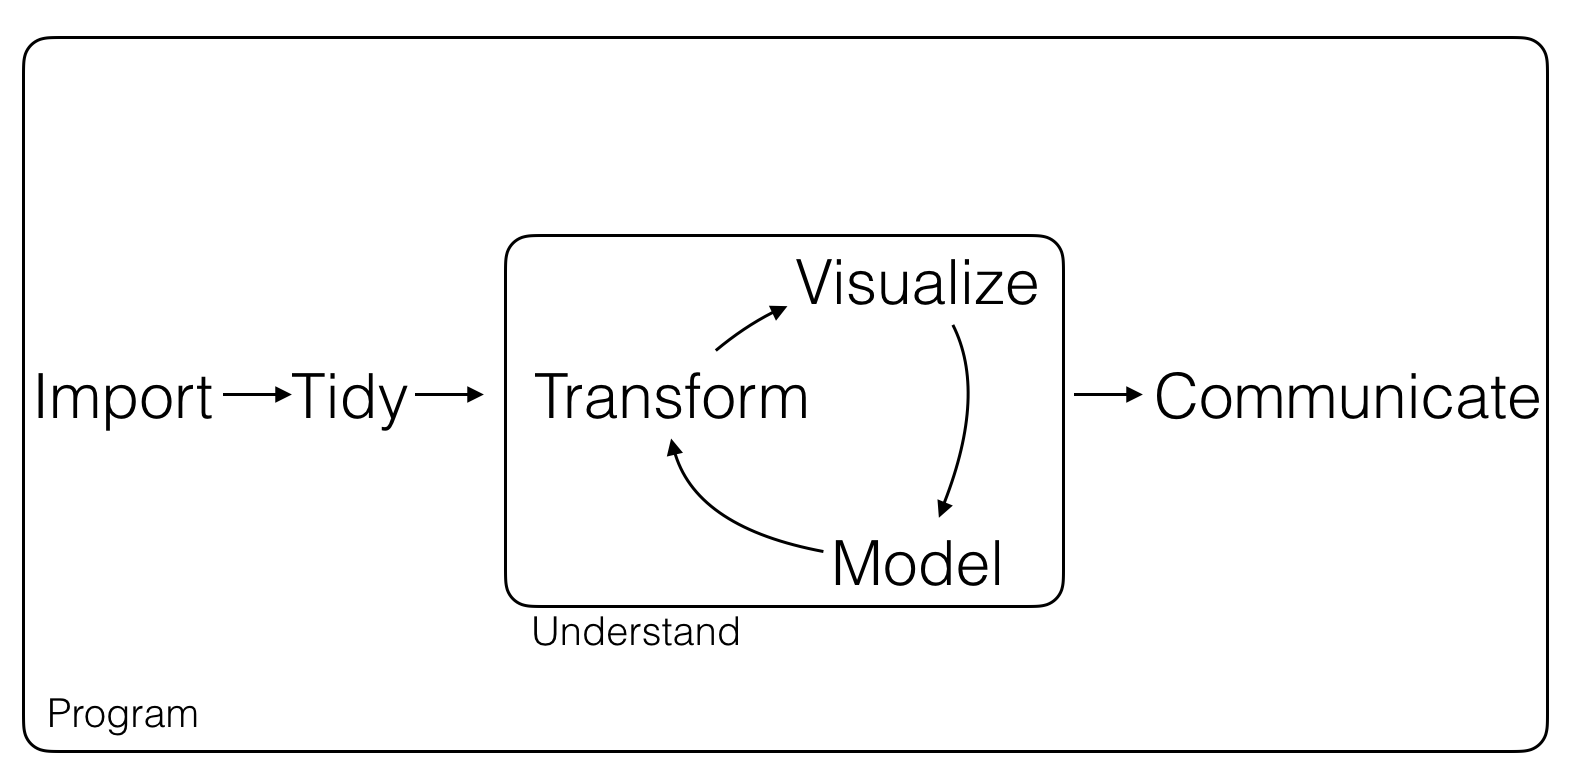
\includegraphics[width=0.8\linewidth]{_bookdown_files/figures/main_work_flow} 

}

\caption{A general workflow for the process of data analysis. Readapted from Wickham (2016)}\label{fig:mainworkflow}
\end{figure}

\section{Challenges: Understanding and
Programming}\label{challenges-understanding-and-programming}

\subsection{Understanding}\label{understanding}

\subsection{Programming}\label{programming}

\section{Research Questions}\label{research-questions}

\section{Stakeholders}\label{stakeholders}

Marketing

Research and Development

Design

Human Resources

Other Stakeholders

\chapter{State of the Art}\label{sota}

The analysis of technical documents require the design of processes that
rely both on programming and Natural Language Processing techniques and
on the undestanding and knowldege of field experts. While the first
techniques are codified and explicit, the second are sometimes implicit
and always harder to systematize. In this section i treat these two
groups of techniques in the same way to give to the reader a sistematic
litterature review on these topics. For this reason the sections of this
chapter has the sequent structure:

\begin{itemize}
\tightlist
\item
  At a first level we have two sections \ref{sotatools} and
  \ref{sotadocuments}, reviewing respectivelly the processes of
  \emph{programming and Natural Language Processing} and of
  \emph{undestanding and knowldege of field experts application};
\item
  Section \ref{sotatools} has a subsection for each of the \emph{phases}
  showed in figure tot. These subsections goes from
  \ref{sotatoolsprogram} to \ref{sotatoolscomunicate};
\item
  Each subsection from \ref{sotatoolsprogram} to
  \ref{sotatoolscomunicate} contains the relative Natural Language
  Processing \emph{task} that are relevant for the analysis of technical
  documents, for example Document Retrieval
  \ref{sotatoolsimportretrieval}, Part-Of-Speech-Tagging;
  \ref{sotatoolstransformpos} or Named Entity Recognition
  \ref{sotatoolsmodelner}.
\item
  Each task subsection describes the relevant \emph{techniques} to
  perform that task. I use the word techniques to include mainly
  algorythms and procedures but also more generic methods or frameworks;
\item
  Since the second section \ref{sotadocuments} describes less
  systematics phases, task and techniques this section opens with a
  first subsection \ref{sotadocumentsunderstand} that focuses on the
  studies of the problems of using expert knowledge in an analytical
  process and which are the techniques to convert this knowledge in a
  format that is usable in a Natural Language Processing workflow.
\item
  Finally, always section \ref{sotadocuments} has a subsection for each
  of the technical \emph{documents} I analyzed (aggiungi gancio con
  introduzione). These subsections goes from \ref{sotadocumentspatents}
  to \ref{sotadocumentsjobs}.
\end{itemize}

\section{Phases, Tasks, and Techniques}\label{sotatools}

In this section I make a review of the most important techniques for
Natural Language Processing. The techniques (mainly algorythms) are
grouped in phases (Import, Tidy, Transform, Model, Visualize,
Communicate) showed in figure \ref{fig:mainworkflow} and each phases is
dived in the NLP tasks that are the most important for the analysis of
technical documents. The algorythm i reviewed in this section are
summmarised in table tot, where the reader can see the relationship
between tasks and techniques.

\subsection{Program}\label{sotatoolsprogram}

\subsection{Import}\label{sotatoolsimport}

\subsubsection{Document Retrieval}\label{sotatoolsimportretrieval}

\subsection{Tidy}\label{sotatoolstidy}

\subsection{Transform}\label{sotatoolstransform}

\subsubsection{Stemming}\label{sotatoolstransformstemming}

\subsubsection{Lemmatisation}\label{sotatoolstransformlemmatisation}

\subsubsection{N-Grams}\label{sotatoolstransformngrams}

\subsubsection{Part-of-Speech Tagging}\label{sotatoolstransformpos}

\subsubsection{Regular Expressions}\label{sotatoolstransformregex}

\subsection{Model}\label{sotatoolsmodel}

\subsubsection{Document Classification}\label{sotatoolsmodeldocclass}

\subsubsection{Network Analysis}\label{sotatoolsmodelnetanal}

\subsubsection{Sentiment Analsysis}\label{sotatoolsmodelsentanal}

\subsubsection{Named Entity Recognition}\label{sotatoolsmodelner}

\subsubsection{Vector Semantics}\label{sotatoolsmodelvec}

\subsubsection{Topic Modelling}\label{sotatoolsmodeltopicmodel}

\subsection{Visualize}\label{sotatoolsvisualize}

\subsection{Comunicate}\label{sotatoolscomunicate}

\section{Documents}\label{sotadocuments}

\subsection{Understand}\label{sotadocumentsunderstand}

Rember to modify the DS workflow

\subsubsection{The problem of byases}\label{sotadocumentsunderstandbyas}

\subsubsection{The Importance of Lexicons for Technical Documents
Analysis}\label{sotadocumentsunderstandlexicons}

\subsection{Patents}\label{sotadocumentspatents}

\subsection{Papers}\label{sotadocumentspapers}

\subsection{Projects}\label{sotadocumentsprojects}

\subsection{Wikipedia}\label{sotadocumentswiki}

\subsection{Twitter}\label{sotadocumentstwitter}

\subsection{Job Profiles}\label{sotadocumentsjobs}

\chapter{Methods}\label{methods}

In this chapter I describe the methods applied for the analysis of
different types of documents containing technical information. The
methods are ensamble of Natural Language Processing (NLP) and Text
Mining techniques described in @ref(sota\_tools), re-designed depending
on the analyzed document and the analysis goal.

Table tot summarise the relations between the documents under analysis
(introduced in section @ref(sota\_documents)) and the NLP techniques.

Table documents vs tools

Table algorithms vs tools

\section{Patents}\label{patents}

\section{Papers}\label{papers}

\section{Projects}\label{projects}

\section{Wikipedia}\label{wikipedia}

\section{Twitter}\label{twitter}

\section{Job Profiles}\label{job-profiles}

\chapter{Applications and Results}\label{applications-and-results}

Some \emph{significant} applications are demonstrated in this chapter.

\section{Patents}\label{patents-1}

\section{Papers}\label{papers-1}

\section{Projects}\label{projects-1}

\section{Wikipedia}\label{wikipedia-1}

\section{Twitter}\label{twitter-1}

\section{Job Profiles}\label{job-profiles-1}

\chapter{Future Developments}\label{future-developments}

\section{Marketing}\label{marketing}

\section{Research and Development}\label{research-and-development}

\section{Design}\label{design}

\section{Human Resources}\label{human-resources}

\chapter{Conclusions}\label{conclusions}

We have finished a nice thesis

\bibliography{bib\_book.bib,bib\_papers.bib,bib\_web.bib,bib\_packages.bib}


\end{document}
